\chapter{Dao động tử, số chiếm và trường lượng tử đầu tiên}

Lý thuyết trường lượng tử là khuôn khổ của chúng ta để mô tả hầu như toàn bộ vật lý phi hấp dẫn đã biết. Không nên nhầm khẳng định đó với việc cho rằng có thể giải mọi bài toán. Nguyên tử hydro còn xử lý được; đến một nguyên tử như bo, phép tính đã khó hơn nhiều, còn một con người thì vượt xa mọi phép tính lý thuyết trường khả thi. Khuôn khổ này có thể là nền tảng, nhưng các phương trình của nó vẫn cực kỳ khó giải.

Vì vậy, ta sẽ bắt đầu theo cách sơ cấp nhất có thể. Chủ đề này đôi khi được gọi là \emph{lượng tử hóa lần thứ hai}, nhưng tên gọi ấy sẽ chưa có nhiều ý nghĩa cho đến khi ta xây dựng xong bộ công cụ cần thiết. Con đường ngắn nhất không bắt đầu từ một trường tương đối tính, mà từ dao động tử điều hòa. Lò xo không phải là điều cốt yếu. Điều quan trọng là đại số của các toán tử nâng và hạ. Khi lặp lại đại số ấy cho nhiều mode, toán tử nâng sẽ không còn chỉ có nghĩa là ``nâng dao động tử lên một mức'' mà sẽ thực sự có nghĩa là ``tạo ra một hạt.''

\section{Dao động tử dưới góc nhìn đại số}

Với một dao động tử, ký hiệu \(a^\dagger\) là toán tử nâng kích thích, còn \(a\) là toán tử hạ kích thích. Các ký hiệu \(a_+\) và \(a_-\) cũng tương đương, nhưng ký hiệu dấu dagger báo trước cách viết dùng trong lý thuyết trường. Trạng thái đáy thỏa mãn
\begin{equation}
a|0\rangle=0,
\end{equation}
và toán tử số là
\begin{equation}
N=a^\dagger a,
\qquad
N|n\rangle=n|n\rangle.
\end{equation}
Hai toán tử bậc thang là liên hợp Hermite của nhau, và hệ thức giao hoán cốt yếu của chúng là
\begin{equation}
[a,a^\dagger]=1.
\label{eq:l06-single-commutator}
\end{equation}
Đại số nhỏ bé này gần như đã bao quát toàn bộ dao động tử.

Có thể biểu diễn \(a\) và \(a^\dagger\) bằng các tổ hợp tuyến tính thích hợp của vị trí và động lượng. Quy ước cụ thể phụ thuộc vào cách chuẩn hóa \(x\), \(p\), \(m\) và \(\omega\); phát biểu bất biến hữu ích ở đây là \(a^\dagger a\) dựng lại Hamilton của dao động tử bậc hai, ngoại trừ năng lượng điểm không cộng thêm. Do đó
\begin{equation}
H=\hbar\omega\left(N+\frac12\right).
\end{equation}
Trong phần thảo luận này, ta bỏ số hạng hằng và xét
\begin{equation}
H=\hbar\omega N.
\label{eq:l06-one-oscillator-hamiltonian}
\end{equation}
Tần số cho biết cái giá của một kích thích. Nâng \(n\) thêm một mức tốn \(\hbar\omega\); hạ \(n\) một mức giải phóng đúng chừng ấy năng lượng.

\section{Nhiều dao động tử độc lập}

Bây giờ xét nhiều dao động tử và đánh nhãn chúng bằng \(i\). Nhãn này chỉ là một chỉ số, không phải đơn vị ảo. Có thể có hữu hạn hoặc vô hạn mode. Một tập hợp các lò xo độc lập là một hình dung; các mode riêng của dây đàn vĩ cầm lý tưởng là một hình dung khác. Trong các ứng dụng lý thuyết trường, trường hợp có vô hạn mode mới là trường hợp quan trọng.

Tính độc lập có ý nghĩa về mặt toán tử. Các toán tử thuộc về những hệ con thực sự độc lập thì giao hoán với nhau. Nếu không, các đại lượng tương ứng không thể được đo độc lập, và ngay từ đầu các hệ ấy đã không độc lập. Vì vậy, ta có
\begin{align}
[a_i,a_j]&=0, \\
[a_i^\dagger,a_j^\dagger]&=0, \\
[a_i,a_j^\dagger]&=\delta_{ij}.
\label{eq:l06-many-commutators}
\end{align}
Khi \(i\ne j\), mọi thứ thuộc về hai mode đều giao hoán. Khi \(i=j\), dòng cuối rút gọn thành Phương trình~\eqref{eq:l06-single-commutator}.

Mỗi dao động tử có toán tử số riêng và, nói chung, tần số riêng:
\begin{equation}
N_i=a_i^\dagger a_i,
\qquad
H=\sum_i\hbar\omega_i N_i.
\label{eq:l06-many-hamiltonian}
\end{equation}
Một trạng thái riêng đồng thời được đánh nhãn bằng danh sách đầy đủ
\begin{equation}
|n_1,n_2,n_3,\ldots\rangle,
\qquad n_i=0,1,2,\ldots.
\label{eq:l06-occupation-ket}
\end{equation}
Số nguyên \(n_i\) được gọi là \emph{số chiếm} của dao động tử thứ \(i\). Ở giai đoạn này, đó chỉ là thuật ngữ. Chẳng bao lâu nữa, nó sẽ đếm số hạt chiếm một trạng thái một hạt, và tên gọi ấy sẽ đúng theo nghĩa đen.

Trạng thái có mọi số chiếm bằng không là
\begin{equation}
|0\rangle\equiv|0,0,0,\ldots\rangle,
\qquad a_i|0\rangle=0\quad\text{for every }i.
\label{eq:l06-oscillator-vacuum}
\end{equation}

\begin{classroomqa}\lecturetimestamp{00:15:27}\audiencequestion{Một họ dao động tử vô hạn có tương ứng với liên tục các mode của một hệ như dây đàn vĩ cầm không?}\lecturerresponse{Có, đối với dây lý tưởng. Dây thực được cấu tạo từ các nguyên tử, nên các bước sóng đủ ngắn cuối cùng sẽ gặp một ngưỡng cắt vi mô. Dù vậy, mô hình liên tục vẫn gợi ý cho ta tập hợp vô hạn mode được dùng trong lý thuyết trường.}\end{classroomqa}

\section{Vì sao các hệ số bậc thang là căn bậc hai}

Tác dụng của \(a^\dagger\) phải nâng trạng thái riêng của \(N\) lên trạng thái riêng kế tiếp, nhưng điều kiện chuẩn hóa vẫn cho phép có một hệ số:
\begin{equation}
a^\dagger|n\rangle=c_n|n+1\rangle.
\label{eq:l06-unknown-coefficient}
\end{equation}

\begin{figure}[htbp]\centering
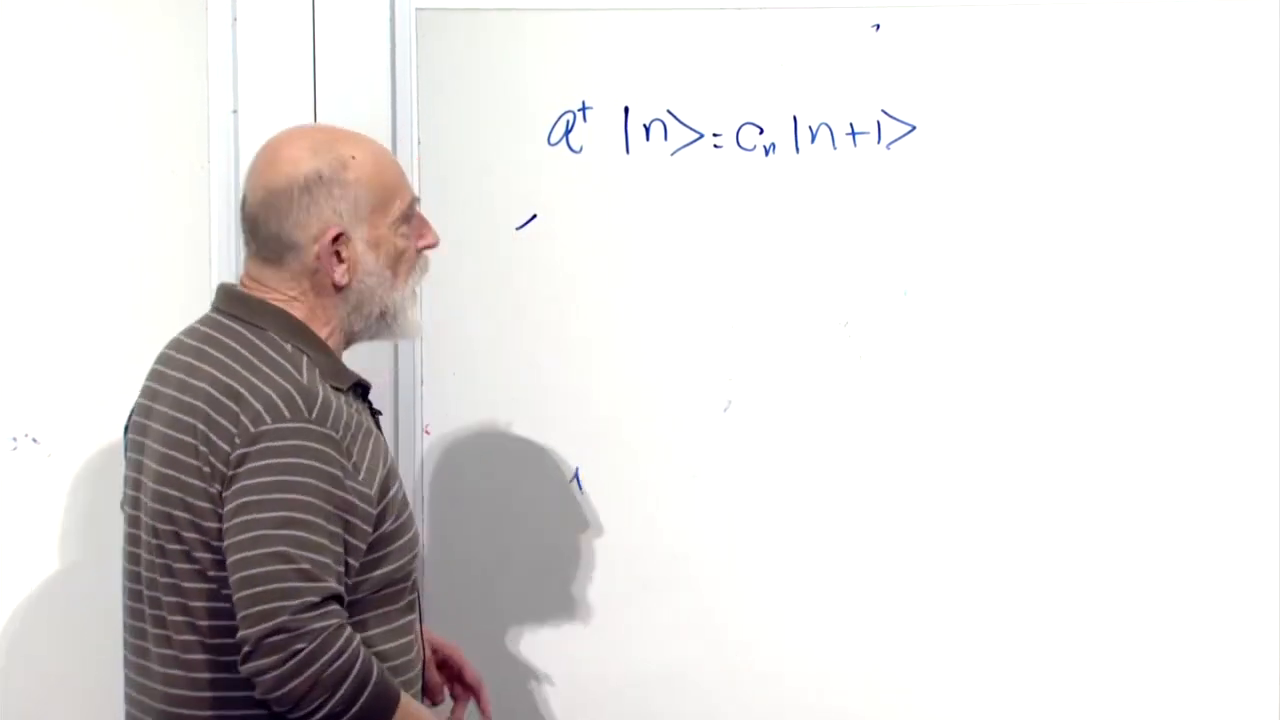
\includegraphics[width=0.9\linewidth]{lecture_06_frame_01.png}\caption{Hệ số bậc thang được đưa vào trước khi suy ra cách chuẩn hóa của nó. Phương trình trên bảng được chép lại trong Phương trình~\eqref{eq:l06-unknown-coefficient}}\lectureframe{00:19:38}\end{figure}

Chọn quy ước pha sao cho \(c_n\) là số thực. Lấy liên hợp Hermite, ta được
\begin{equation}
\langle n|a=c_n\langle n+1|.
\end{equation}
Nhân hai hệ thức với nhau và dùng các trạng thái cơ sở đã chuẩn hóa,
\begin{align}
c_n^2
&=\langle n|aa^\dagger|n\rangle \\
&=\langle n|(a^\dagger a+1)|n\rangle \\
&=\langle n|(N+1)|n\rangle \\
&=n+1.
\end{align}
Suy ra
\begin{equation}
a^\dagger|n\rangle=\sqrt{n+1}\,|n+1\rangle.
\label{eq:l06-raising-rule}
\end{equation}

\begin{classroomqa}\lecturetimestamp{00:22:35}\audiencequestion{Vì sao có thể đặt \(\langle n+1|n+1\rangle=1\) trước khi tìm \(c_n\)}\lecturerresponse{Ngay từ đầu, các vectơ riêng được chọn làm một cơ sở đã chuẩn hóa. Điều kiện chuẩn hóa của chúng không xác định chuẩn hóa của \(a^\dagger|n\rangle\); thông tin còn thiếu ấy chính là hệ số \(c_n\)}\end{classroomqa}

Quy tắc hạ được suy ra tương tự:
\begin{equation}
a|n\rangle=\sqrt n\,|n-1\rangle.
\label{eq:l06-lowering-rule}
\end{equation}
Khi \(n=0\), hệ số tự động triệt tiêu, nên quy tắc này bao gồm cả trường hợp \(a|0\rangle=0\). Với nhiều mode, toán tử chỉ thay đổi số chiếm ở vị trí tương ứng với chính nó:
\begin{align}
a_i^\dagger|n_1,\ldots,n_i,\ldots\rangle
&=\sqrt{n_i+1}\,|n_1,\ldots,n_i+1,\ldots\rangle, \\
a_i|n_1,\ldots,n_i,\ldots\rangle
&=\sqrt{n_i}\,|n_1,\ldots,n_i-1,\ldots\rangle.
\label{eq:l06-multimode-ladders}
\end{align}
Các số chiếm khác không thay đổi.

\section{Hàm sóng không phải là trường lượng tử}

Trước khi định nghĩa trường, ta cần phân biệt nó với hàm sóng quen thuộc. Ba điểm tương phản sẽ dẫn dắt bước chuyển này.

Thứ nhất, hàm sóng của một hạt
\begin{equation}
\psi(x)=\langle x|\psi\rangle
\end{equation}
là một biểu diễn của vectơ trạng thái. Bản thân nó không phải là một đại lượng có thể quan sát. Ta đo vị trí, động lượng, mômen động lượng và các toán tử khác; hàm sóng cung cấp các biên độ dùng để tính xác suất nhận được những kết quả ấy.

Thứ hai, hàm sóng của nhiều hạt phụ thuộc vào vị trí của tất cả các hạt. Với hai hạt có các vectơ vị trí tạm gọi là \(x\) và \(y\),
\begin{equation}
\psi(x,y)=\langle x,y|\psi\rangle.
\end{equation}
Ở đây, \(x\) và \(y\) lần lượt chỉ hai hạt khác nhau; chúng không phải là các thành phần Cartesian thứ \(x\) và thứ \(y\) của cùng một vectơ vị trí. Với \(N\) hạt, trạng thái được biểu diễn bằng
\begin{equation}
\psi(x_1,x_2,\ldots,x_N).
\end{equation}

Thứ ba, hàm sóng này mô tả một số hạt cố định. Hàm sóng của mười lăm hạt có mười lăm đối số vị trí và thuộc về không gian Hilbert của mười lăm hạt. Tự nó, hàm sóng ấy không mô tả một quá trình trong đó số hạt thay đổi từ mười lăm thành mười bốn hoặc mười sáu.

Trường lượng tử đảo ngược những đặc điểm này. Nó là một toán tử chứ không phải một trạng thái, phụ thuộc vào một điểm không gian \(x\), và tác dụng lên một không gian trạng thái chứa mọi sector số hạt. Cụm từ ``một điểm'' có nghĩa là một vectơ vị trí biến thiên tự do. Không có nghĩa là \(x\) đã được gán một giá trị số cụ thể.

Có một điều cần lưu ý, sau này sẽ quan trọng. Trường \(\Psi(x)\) được giới thiệu dưới đây không Hermite, nên theo nghĩa nghiêm ngặt, bản thân nó không phải là đại lượng có thể quan sát. Các tổ hợp Hermite của nó mới là đại lượng có thể quan sát. Vì vậy, phát biểu tạm thời rằng trường có thể đo được được làm chính xác hơn chứ không bị bác bỏ: trường là các hàm nhận giá trị toán tử, còn các tổ hợp Hermite của chúng biểu diễn những đại lượng có thể đo.

\begin{classroomqa}\lecturetimestamp{00:36:52}\audiencequestion{Nếu trường là hàm của một vị trí, vị trí đó có thể biến thiên không? Và \(y\) trong hàm sóng hai hạt đã đi đâu?}\lecturerresponse{Điểm \(x\) biến thiên trên khắp không gian. ``Một vị trí'' có nghĩa là toán tử có một đối số không gian, chứ không phải đối số ấy cố định. Trong \(\psi(x,y)\), các ký hiệu \(x\) và \(y\) chỉ vị trí của hai hạt; tương đương, chúng là \(x_1\) và \(x_2\). Chúng không phải là hai thành phần Cartesian của đối số trường.}\end{classroomqa}

\begin{classroomqa}\lecturetimestamp{00:38:15}\audiencequestion{Hàm sóng của số hạt cố định và cách mô tả bằng trường liên hệ với nhau thế nào, và chúng có mô tả những loại hạt khác nhau không?}\lecturerresponse{Mối liên hệ ấy là cấu trúc cốt lõi sẽ được xây dựng tiếp theo. Các hạt là cùng một loại. Trong bài giảng này, chúng là boson; fermion đòi hỏi một đại số khác.}\end{classroomqa}

\section{Một hạt trong hộp}

Tạm thời quay lại cơ học lượng tử thông thường của một hạt. Đặt một hạt vào hộp một chiều. Khi chỉ có một hạt, sự phân biệt giữa boson và fermion không liên quan: không có hạt giống hệt thứ hai để xét phép hoán đổi hoặc nguyên lý loại trừ.

Gọi
\begin{equation}
\psi_1(x),\ \psi_2(x),\ \psi_3(x),\ldots
\end{equation}
là các hàm riêng năng lượng. Mode thấp nhất là sóng trơn nhất triệt tiêu ở hai vách. Mode kế tiếp có một nút bên trong, còn các mode năng lượng cao hơn dao động nhanh hơn. Trong giếng vuông vô hạn lý tưởng có chiều rộng \(L\), một cơ sở trực chuẩn đã chuẩn hóa thuận tiện là
\begin{equation}
\psi_i(x)=\sqrt{\frac{2}{L}}\sin\!\left(\frac{i\pi x}{L}\right),
\qquad 0<x<L.
\label{eq:l06-box-basis}
\end{equation}
Công thức sin tường minh là một ví dụ chuẩn cho hình phác họa định tính trên bảng; lập luận dưới đây chỉ cần một tập đầy đủ các trạng thái một hạt trực chuẩn.

\begin{figure}[htbp]\centering
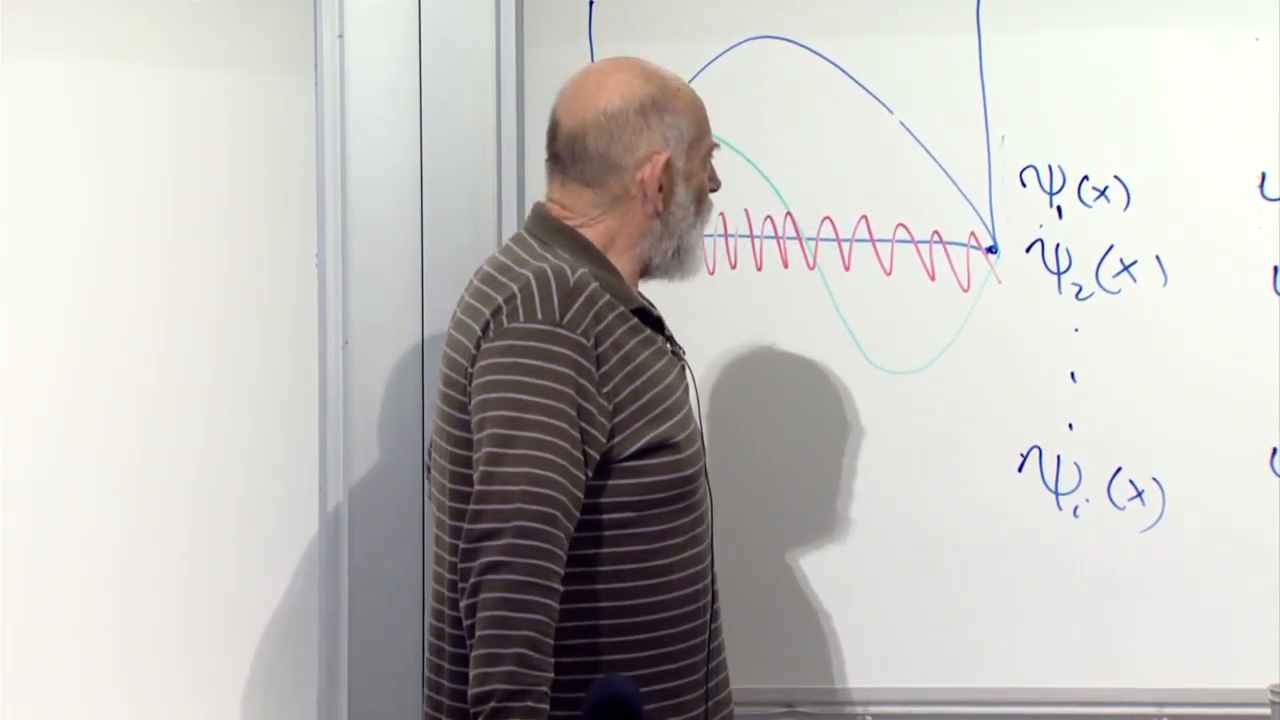
\includegraphics[width=0.9\linewidth]{lecture_06_frame_03.png}\caption{Các mode của hạt trong hộp, sắp theo năng lượng tăng dần. Mode đầu tiên không có nút bên trong, mode thứ hai có một nút, còn các mode bậc cao bị lược đi dao động ngày càng nhanh.}\lectureframe{00:43:10}\end{figure}

Có thể vẽ lại cấu trúc ấy mà không bị hình ảnh trên bảng trực tiếp che khuất:
\begin{figure}[htbp]\centering
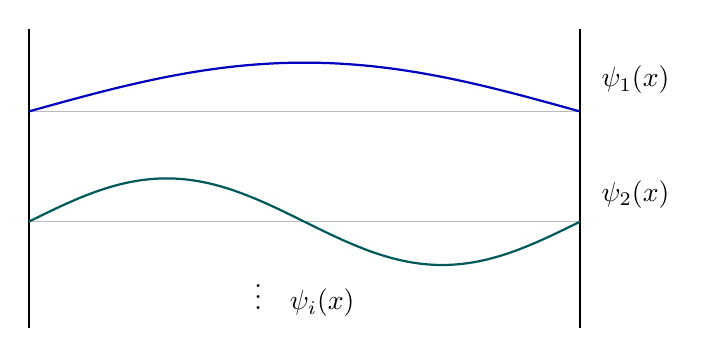
\begin{tikzpicture}[x=1cm,y=1cm]
  \draw[thick] (0,0) -- (0,3.8);
  \draw[thick] (7,0) -- (7,3.8);
  \draw[gray!55] (0,2.75) -- (7,2.75);
  \draw[gray!55] (0,1.35) -- (7,1.35);
  \draw[blue!75!black,thick,domain=0:7,samples=120]
    plot (\x,{2.75+0.62*sin(180*\x/7)});
  \draw[teal!70!black,thick,domain=0:7,samples=120]
    plot (\x,{1.35+0.55*sin(360*\x/7)});
  \node[right] at (7.15,3.15) {$\psi_1(x)$};
  \node[right] at (7.15,1.70) {$\psi_2(x)$};
  \node at (3.5,0.45) {$\vdots\quad \psi_i(x)$};
\end{tikzpicture}\caption{Bản dựng lại rõ ràng của hình phác họa định tính các mode trong hộp. Độ dịch theo phương đứng giúp tách các hàm riêng cho dễ nhìn, không phải là một tọa độ vật lý bổ sung.}\end{figure}

Chỉ số \(i\) đánh nhãn một trạng thái một hạt, không phải một hạt và cũng không phải số nút. Với cơ sở trong hộp, \(i\) tình cờ bằng số nút bên trong cộng một. Mỗi trạng thái có năng lượng \(\varepsilon_i\). Theo ký hiệu của bài giảng, ta có thể viết năng lượng này là \(\hbar\omega_i\), hoặc đơn giản là \(\omega_i\) sau khi đặt \(\hbar=1\).

\begin{classroomqa}\lecturetimestamp{00:39:01}\audiencequestion{Giả thiết về tính độc lập trước đó có chính xác không, và chỉ số \(i\) có thể đánh nhãn các trạng thái khả dĩ của electron trong nguyên tử không?}\lecturerresponse{Trong cấu trúc các mode độc lập, các hệ thức giao hoán giữa những mode khác nhau là chính xác. Chỉ số này có thể đánh nhãn các trạng thái một hạt trong nguyên tử. Tuy nhiên, nếu các hạt tương tác thì Hamilton đơn giản của các mode độc lập không còn mô tả đầy đủ hệ nữa.}\end{classroomqa}

\begin{classroomqa}\lecturetimestamp{00:40:34}\audiencequestion{Hạt trong hộp có phải là boson không?}\lecturerresponse{Có thể là boson, nhưng với một hạt thì thống kê không quan trọng. Nguyên lý loại trừ và phép hoán đổi chỉ có ý nghĩa khi có nhiều hơn một hạt giống hệt nhau.}\end{classroomqa}

\section{Từ các mode trong hộp đến không gian Fock}

Bây giờ cho phép có số boson giống hệt nhau bất kỳ trong hộp. Một số \(n_1\) hạt có thể chiếm \(\psi_1\), một số \(n_2\) hạt có thể chiếm \(\psi_2\), vân vân. Vì thế, một trạng thái cơ sở có dạng
\begin{equation}
|n_1,n_2,n_3,\ldots\rangle.
\end{equation}
Đây chính xác là ký hiệu đã dùng cho nhiều dao động tử. Sự tương ứng mang tính cấu trúc: gán một dao động tử cho mỗi trạng thái một hạt, rồi đồng nhất số kích thích của dao động tử với số hạt chiếm trạng thái ấy.

Boson là điều thiết yếu ở đây vì mỗi \(n_i\) có thể là bất kỳ số nguyên không âm nào. Với fermion, mỗi trạng thái một hạt chỉ có thể để trống hoặc được chiếm bởi một hạt, tuyệt đối không thể bị chiếm bởi hai hạt; vì vậy không thể giữ nguyên đại số dao động tử thông thường.

Giờ đây, có thể định nghĩa các toán tử thông qua tác dụng của chúng lên cơ sở số chiếm. Toán tử \(a_i^\dagger\) tạo ra một hạt trong trạng thái một hạt \(i\); toán tử \(a_i\) loại bỏ một hạt:
\begin{align}
a_i^\dagger|n_1,\ldots,n_i,\ldots\rangle
&=\sqrt{n_i+1}\,|n_1,\ldots,n_i+1,\ldots\rangle, \\
a_i|n_1,\ldots,n_i,\ldots\rangle
&=\sqrt{n_i}\,|n_1,\ldots,n_i-1,\ldots\rangle.
\end{align}
Đây không phải là phép ví von được đưa ra sau đó. Đó là định nghĩa của các toán tử tạo và hủy boson trên cơ sở này. Vì cơ sở sinh ra toàn bộ không gian, định nghĩa này xác định tác dụng của chúng lên mọi trạng thái nhờ tính tuyến tính.

\begin{classroomqa}\lecturetimestamp{00:47:11}\audiencequestion{\(n_1,n_2,n_3\) có phải là các trạng thái lượng tử không?}\lecturerresponse{Các nhãn \(1,2,3,\ldots\) xác định các trạng thái một hạt. Các ký hiệu \(n_1,n_2,n_3,\ldots\) là số hạt chiếm những trạng thái ấy. Giữ phân biệt giữa nhãn trạng thái và số chiếm của nó là yêu cầu ký hiệu chính yếu.}\end{classroomqa}

\subsection{Ý nghĩa của căn bậc hai}

Thừa số \(\sqrt{n_i+1}\) không biểu thị một hạt bổ sung hay một quá trình vật lý riêng biệt. Nó giúp toán tử có chuẩn hóa và đại số chính xác. Với một mode,
\begin{align}
a a^\dagger|n\rangle
&=a\bigl(\sqrt{n+1}\,|n+1\rangle\bigr) \\
&=(n+1)|n\rangle,
\end{align}
trong khi
\begin{equation}
a^\dagger a|n\rangle=n|n\rangle.
\end{equation}
Vì thế, hiệu của chúng là \(|n\rangle\), đúng như yêu cầu của \([a,a^\dagger]=1\). Nói gần đúng, mỗi toán tử bậc thang có độ lớn cỡ \(\sqrt n\), vì tích của chúng cho toán tử số có độ lớn cỡ \(n\).

\begin{classroomqa}\lecturetimestamp{00:47:52}\audiencequestion{Thừa số căn bậc hai có ý nghĩa vật lý cụ thể nào?}\lecturerresponse{Chủ yếu, đó là một hệ số chuẩn hóa toán học. Nó bảo đảm các trạng thái số chiếm được chuẩn hóa, \(a^\dagger a\) có trị riêng \(n\), và các toán tử bậc thang thỏa mãn hệ thức giao hoán của dao động tử. Đôi khi, ý nghĩa ta cần chính là ý nghĩa toán học.}\end{classroomqa}

\begin{classroomqa}\lecturetimestamp{00:52:25}\audiencequestion{Các toán tử tạo và hủy có được định nghĩa chỉ thông qua các tính chất và tác dụng của chúng lên cơ sở không?}\lecturerresponse{Đúng vậy. Định nghĩa không nhất thiết phải xuất phát từ một hình dung cơ bản hơn. Giá trị của chúng được đánh giá qua hệ quả. Định nghĩa tác dụng trên một cơ sở đầy đủ xác định toán tử ở mọi nơi, và các định nghĩa này tái tạo những hệ thức giao hoán mong muốn.}\end{classroomqa}

\begin{classroomqa}\lecturetimestamp{00:53:22}\audiencequestion{Vì sao \(a_i\) làm một hạt biến mất thay vì chỉ chuyển nó sang một trạng thái khác?}\lecturerresponse{Vì \(a_i\) được định nghĩa là làm giảm số chiếm của trạng thái \(i\). Câu hỏi hữu ích không phải là vì sao một định nghĩa đúng, mà là vì sao định nghĩa ấy hữu ích. Nó hữu ích vì phát xạ và hấp thụ đòi hỏi các toán tử làm thay đổi số hạt: photon được tạo ra khi bức xạ phát ra và bị hủy khi được hấp thụ.}\end{classroomqa}

Không gian được sinh bởi mọi trạng thái số chiếm được gọi là \emph{không gian Fock}. Không gian này chứa chân không, mọi trạng thái một hạt, mọi trạng thái hai hạt, vân vân, mà không có giới hạn trên cố định:
\begin{equation}
\mathcal F=\mathcal H_0\oplus\mathcal H_1\oplus\mathcal H_2\oplus\cdots.
\label{eq:l06-fock-space}
\end{equation}
Ký hiệu tổng trực tiếp cho thấy điều mà hàm sóng thông thường của \(N\) hạt không thể hiện: mọi sector số hạt đều thuộc về cùng một không gian trạng thái.

\begin{classroomqa}\lecturetimestamp{00:54:56}\audiencequestion{Định nghĩa các toán tử trên các vectơ riêng số chiếm có xác định được chúng trên các vectơ tùy ý không, và từ đó có suy ra các hệ thức giao hoán của dao động tử không?}\lecturerresponse{Chính xác. Các vectơ chiếm số tạo thành một cơ sở, nên tính tuyến tính mở rộng định nghĩa ra toàn bộ không gian Fock. Tác dụng lên cơ sở này xác nhận các hệ thức giao hoán boson. Mỗi trạng thái một hạt được biểu diễn bằng một dao động tử, và số chiếm của dao động tử ấy là số hạt trong trạng thái đó.}\end{classroomqa}

\subsection{Chân không và Hamilton tự do}

Chân không Fock là trạng thái không có hạt trong bất kỳ trạng thái một hạt nào:
\begin{equation}
|0\rangle=|0,0,0,\ldots\rangle,
\qquad a_i|0\rangle=0.
\end{equation}
Từ \emph{trạng thái cơ bản} có thể gây hiểu nhầm ở đây. Trạng thái \emph{một hạt} thấp nhất là mode \(i=1\); chân không Fock không có hạt, kể cả trong mode ấy. Nếu một hạt chiếm mode thấp nhất, \(a_1\) có thể loại bỏ nó và đưa hệ trở về chân không.

\begin{classroomqa}\lecturetimestamp{00:56:19}\audiencequestion{Chân không được mô tả thế nào bằng ngôn ngữ số chiếm? Trạng thái một hạt thấp nhất có bị chiếm không?}\lecturerresponse{Trong chân không, mọi số chiếm đều bằng không và mọi \(a_i\) đều hủy nó. Mode một hạt thấp nhất không bị chiếm trong chân không. Nếu mode ấy bị chiếm, toán tử hủy tương ứng có thể loại bỏ hạt đó.}\end{classroomqa}

Với các hạt không tương tác, năng lượng toàn phần có tính cộng. Nếu một hạt ở trạng thái \(i\) có năng lượng \(\hbar\omega_i\), thì
\begin{align}
H
&=\sum_i \hbar\omega_i N_i \\
&=\sum_i \hbar\omega_i a_i^\dagger a_i.
\label{eq:l06-free-fock-hamiltonian}
\end{align}
Có hai cách diễn giải tương đương. Đó là tổng năng lượng của các dao động tử, mỗi trạng thái một hạt ứng với một dao động tử. Đồng thời, đó cũng là tổng các năng lượng một hạt, mỗi năng lượng được nhân với số hạt mang năng lượng ấy.

Trong ký hiệu lý thuyết trường, \(a_i^\dagger\) thường được gọi là toán tử tạo, còn \(a_i\) là toán tử hủy. Ký hiệu cũ \(a_+\) và \(a_-\) cũng có cùng ý nghĩa.

\section{Giải đáp trước khi xuất hiện trường}

Một số câu hỏi sau giờ nghỉ giúp phân biệt cách ghi sổ dao động tử mới này với một hạt thông thường chuyển động trong thế năng dao động tử.

\begin{classroomqa}\lecturetimestamp{01:06:09}\audiencequestion{Các mức năng lượng của hạt trong hộp không cách đều nhau, vậy dao động tử điều hòa nằm ở đâu?}\lecturerresponse{Các năng lượng một hạt \(\omega_i\) không nhất thiết cách đều nhau. Tuy nhiên, với mỗi mode cố định \(i\), năng lượng của không, một, hai và ba hạt không tương tác trong mode ấy là \(0,\omega_i,2\omega_i,3\omega_i\). Thang số chiếm đó chính là dao động tử. Nó khác với việc đặt một hạt trong thế năng của dao động tử điều hòa.}\end{classroomqa}

\begin{classroomqa}\lecturetimestamp{01:08:38}\audiencequestion{Cấu trúc này có liên hệ với khai triển Fourier không?}\lecturerresponse{Có, và liên hệ rất sâu sắc. Nếu cơ sở một hạt gồm các mode động lượng, thì các hàm mode là sin, cos hoặc hàm mũ phức, còn các \(a_i\) là những đại lượng tương tự hệ số Fourier trong cơ học lượng tử. Cơ sở tổng quát không nhất thiết phải gồm các hàm lượng giác, nhưng logic khai triển vẫn như nhau.}\end{classroomqa}

\begin{classroomqa}\lecturetimestamp{01:09:07}\audiencequestion{Có phải tất cả các hạt đều được gán cùng một năng lượng, và có tính đến tương tác không?}\lecturerresponse{Các hạt chiếm cùng một trạng thái một hạt có cùng năng lượng, còn các hạt ở những trạng thái khác nhau nói chung có năng lượng khác nhau. Hiện tại, các hạt là tự do: chúng không tương tác. Tương tác sẽ bổ sung các số hạng thế năng, khiến Hamilton không còn chỉ là tổng cộng tính trong Phương trình~\eqref{eq:l06-free-fock-hamiltonian}.}\end{classroomqa}

\begin{classroomqa}\lecturetimestamp{01:10:26}\audiencequestion{Nửa lượng tử năng lượng điểm không trong mỗi dao động tử đã đi đâu?}\lecturerresponse{Đó là một hằng số cộng trong Hamilton. Hằng số giao hoán với mọi toán tử, nên không làm thay đổi các phương trình chuyển động Heisenberg; các phép đo thông thường trong vật lý phi hấp dẫn phụ thuộc vào hiệu năng lượng. Hằng số ấy có thể quan trọng trong những mục đích đặc biệt, nhưng không ảnh hưởng đến cấu trúc đang được xây dựng ở đây.}\end{classroomqa}

Lý thuyết tự do đã là một công cụ ghi sổ có sức mạnh khác thường. Nó theo dõi không chỉ nhiều hạt, mà cả những hạt đổi trạng thái, xuất hiện, biến mất hoặc tồn tại trong chồng chập của các tổng số hạt khác nhau. Các toán tử không chỉ là ký hiệu ghi sổ, vì những tổ hợp Hermite thích hợp của chúng có thể được đo; tuy vậy, ghi sổ vẫn là một trực giác ban đầu hữu ích.

\begin{classroomqa}\lecturetimestamp{01:14:03}\audiencequestion{Lý thuyết trường và lý thuyết trường lượng tử bắt nguồn từ đâu trong lịch sử?}\lecturerresponse{Một phác thảo ngắn về lịch sử bắt đầu với hình dung vật lý của Faraday về điện trường và từ trường, cùng các phương trình Maxwell cho trường cổ điển. Planck đưa ra lượng tử năng lượng khi nghiên cứu bức xạ nhiệt; Einstein đồng nhất sự lượng tử hóa với chính trường điện từ và với lượng tử ánh sáng. Heisenberg, Pauli và đặc biệt là Dirac đã góp phần xây dựng khuôn khổ toán tử hiện đại vào khoảng cuối thập niên 1920. Tai biến tử ngoại và mô tả lượng tử của bức xạ là những vấn đề then chốt thuở ban đầu. Đây là phác thảo lịch sử, không phải bản phân định đầy đủ về quyền ưu tiên.}\end{classroomqa}

Mạch lịch sử cũng giải thích vì sao dao động tử liên tục xuất hiện. Bức xạ cổ điển trong một hốc cộng hưởng có thể khai triển thành các mode riêng. Lượng tử hóa những mode ấy biến số kích thích của chúng thành số photon. Các lượng tử toán học chiếm những mode trở thành các hạt vật lý.

\section{Toán tử trường boson}

Gọi \(\{\psi_i(x)\}\) là một cơ sở đầy đủ trực chuẩn của các hàm sóng một hạt. Định nghĩa
\begin{equation}
\boxed{\Psi(x)=\sum_i a_i\,\psi_i(x)}
\label{eq:l06-field-annihilation}
\end{equation}
và liên hợp Hermite của nó
\begin{equation}
\boxed{\Psi^\dagger(x)=\sum_i a_i^\dagger\,\psi_i^*(x)}.
\label{eq:l06-field-creation}
\end{equation}

\begin{figure}[htbp]\centering
\includegraphics[width=0.9\linewidth]{lecture_06_frame_04.png}\caption{Các khai triển mode đầy đủ của trường hủy và liên hợp Hermite của nó. Các Phương trình~\eqref{eq:l06-field-annihilation} và \eqref{eq:l06-field-creation} giữ nguyên cấu trúc toán tử và liên hợp phức khi được trình bày dưới dạng sắp chữ.}\lectureframe{01:25:15}\end{figure}

Với mỗi vị trí cố định \(x\), mỗi \(\psi_i(x)\) là một số phức thông thường. Toàn bộ nội dung toán tử nằm trong \(a_i\) và \(a_i^\dagger\). Khi \(x\) biến thiên, ta thu được một toán tử khác nhau tại mỗi điểm trong không gian. Đó chính là ý nghĩa chính xác của việc \(\Psi\) là một hàm nhận giá trị toán tử.

Nếu các hàm cơ sở là sóng phẳng, các Phương trình~\eqref{eq:l06-field-annihilation} và \eqref{eq:l06-field-creation} là những khai triển Fourier lượng tử: các hệ số Fourier cổ điển đã trở thành toán tử. Trong một chiếc hộp, thay vào đó, cơ sở có thể là các hàm sin trong Phương trình~\eqref{eq:l06-box-basis}. Mọi cơ sở một hạt đầy đủ và trực chuẩn đều dùng được.

Cả \(\Psi\) lẫn \(\Psi^\dagger\) đều không Hermite. Có thể xây dựng các trường quan sát được từ những tổ hợp Hermite như
\begin{equation}
\Psi(x)+\Psi^\dagger(x),
\qquad
i\bigl(\Psi^\dagger(x)-\Psi(x)\bigr),
\end{equation}
và sau này sẽ xây dựng các mật độ quan sát được từ những tích như \(\Psi^\dagger(x)\Psi(x)\). Trước hết, ta cần hiểu hai trường cơ bản này làm gì.

\begin{classroomqa}\lecturetimestamp{01:23:14}\audiencequestion{Làm thế nào vế trái lại có thể là toán tử khi các hàm mode ở vế phải là những hàm sóng thông thường?}\lecturerresponse{Khi đã chọn \(x\), các hàm \(\psi_i(x)\) là những số. Các thừa số \(a_i\) là toán tử. Một số nhân với một toán tử vẫn là toán tử, nên tổng cũng là toán tử. Khi \(x\) biến thiên, ta có cả họ toán tử.}\end{classroomqa}

\section{Trường làm gì}

Trường hủy tác dụng lên chân không lập tức cho kết quả triệt tiêu:
\begin{equation}
\Psi(x)|0\rangle
=\sum_i\psi_i(x)a_i|0\rangle
=0.
\label{eq:l06-field-kills-vacuum}
\end{equation}
Trường tạo cho ta biết nhiều điều hơn hẳn.

Gọi \(|i\rangle\) là trạng thái một hạt có hàm sóng
\begin{equation}
\langle x|i\rangle=\psi_i(x).
\end{equation}
Tính đầy đủ của cơ sở một hạt cho ta
\begin{equation}
\sum_i|i\rangle\langle i|=1.
\label{eq:l06-completeness}
\end{equation}
Áp dụng đồng nhất thức này lên một trạng thái riêng vị trí:
\begin{align}
|x\rangle
&=\sum_i|i\rangle\langle i|x\rangle \\
&=\sum_i\psi_i^*(x)|i\rangle.
\label{eq:l06-position-expansion}
\end{align}
Trong ngôn ngữ Fock, một trạng thái mode một hạt là
\begin{equation}
|i\rangle=a_i^\dagger|0\rangle.
\end{equation}
Thế biểu thức này vào Phương trình~\eqref{eq:l06-position-expansion},
\begin{align}
|x\rangle
&=\sum_i\psi_i^*(x)a_i^\dagger|0\rangle \\
&=\Psi^\dagger(x)|0\rangle.
\label{eq:l06-local-creation}
\end{align}
Vì vậy, \(\Psi^\dagger(x)\) tạo ra một hạt định xứ tại \(x\), còn \(\Psi(x)\) loại bỏ một hạt tại đó. Trạng thái riêng vị trí được định xứ theo hàm delta và là một trạng thái tổng quát, không chuẩn hóa được; muốn có hạt định xứ vật lý, ta lấy trường trung bình theo một gói sóng chuẩn hóa được.\editorialnote{Bài giảng dùng cách diễn đạt lý tưởng bằng trạng thái riêng vị trí. Lưu ý về gói sóng ghi nhận ý nghĩa toán học chuẩn mà không làm thay đổi lập luận.}

\begin{classroomqa}\lecturetimestamp{01:36:26}\audiencequestion{Thông tin xác định loại hạt được tạo ra nằm ở đâu? Trạng thái tại \(x\) có được định xứ theo hàm delta không?}\lecturerresponse{Mỗi loài hạt được gán một trường riêng, nên danh tính của hạt được xác định bởi trường được dùng. Đối số \(x\) xác định vị trí hạt được tạo ra. Trong cơ sở vị trí lý tưởng, trạng thái được tạo ra có độ định xứ theo hàm delta.}\end{classroomqa}

Các ví dụ về loài boson gồm photon, graviton, boson Higgs và gluon, dù các trường thực tế còn mang những chỉ số nội tại. Ngay cả photon cũng cần nhãn phân cực. Ký hiệu trường vô hướng giản lược lược bỏ các nhãn bổ sung ấy để nguyên lý tạo hạt vẫn được thể hiện rõ.

\subsection{Chân không không phải là vectơ không}

Phương trình
\begin{equation}
\Psi(x)|0\rangle=0
\end{equation}
chứa hai đối tượng rất khác nhau cùng được ký hiệu bằng số không. Ket \(|0\rangle\) là chân không: một trạng thái vật lý đã chuẩn hóa, với
\begin{equation}
\langle0|0\rangle=1.
\end{equation}
Kết quả ở vế phải là vectơ không. Chuẩn của nó bằng không; không thể chuẩn hóa nó, và nó không biểu diễn một trạng thái vật lý.

Sự khác nhau trở nên rõ rệt khi xét phép cộng. Cộng vectơ không vào một trạng thái một hạt thì trạng thái không đổi. Cộng chân không vào một trạng thái một hạt thì ta được một chồng chập thực sự của các sector có số hạt khác nhau. Với các hệ số đã chuẩn hóa,
\begin{equation}
|\chi\rangle=\frac{1}{\sqrt2}\bigl(|0\rangle+|1\rangle\bigr)
\end{equation}
có xác suất bằng nhau để có không hạt hoặc một hạt. Trạng thái này không giống \(|1\rangle\).

\begin{classroomqa}
\lecturetimestamp{01:37:23}
\audiencequestion{Nếu không có hạt nào tại \(x\), thì \(\Psi(x)\) có đơn giản là không làm gì không? Kết quả bằng không có nghĩa là gì?}
\lecturerresponse{Nó không trả về trạng thái ban đầu mà trả về vectơ không. Chân không là một trạng thái đã chuẩn hóa, mô tả không gian trống; vectơ không có độ dài bằng không và không mô tả trạng thái vật lý nào. Mọi toán tử tác dụng lên vectơ không đều trả về vectơ không.}
\end{classroomqa}

\begin{classroomqa}
\lecturetimestamp{01:39:00}
\audiencequestion{Điều gì xảy ra nếu cộng chân không, thay vì vectơ không, vào một trạng thái một hạt?}
\lecturerresponse{Ta thu được một chồng chập có biên độ ứng với các số hạt khác nhau. Ngược lại, cộng vectơ không không làm thay đổi trạng thái một hạt. Ký hiệu \(|0\rangle\) chỉ trạng thái không có hạt; nó không có nghĩa là vectơ không.}
\end{classroomqa}

\begin{classroomqa}
\lecturetimestamp{01:41:56}
\audiencequestion{Trong khai triển trường, thứ tự giữa hàm mode và toán tử sinh hoặc hủy có quan trọng không? Các hàm mode có giá trị phức không?}
\lecturerresponse{Hàm mode là một số thông thường nên giao hoán với mọi toán tử; vì vậy thứ tự không quan trọng. Nói chung, các hàm mode có thể nhận giá trị phức; một cơ sở được chọn là thực hay phức tùy thuộc vào bài toán Schr\"odinger một hạt.}
\end{classroomqa}

\subsection{Sự xuất hiện của tính đối xứng boson cho hai hạt}

Để tạo một hạt tại \(x\) và một hạt khác tại \(y\), ta tác dụng hai lần:
\begin{equation}
|x,y\rangle
=\Psi^\dagger(y)\Psi^\dagger(x)|0\rangle.
\label{eq:l06-two-particle-state}
\end{equation}
Hai điểm có thể trùng nhau hoặc khác nhau. Vì các toán tử sinh cơ bản giao hoán với nhau,
\begin{align}
[\Psi^\dagger(x),\Psi^\dagger(y)]
&=\sum_{i,j}\psi_i^*(x)\psi_j^*(y)
[a_i^\dagger,a_j^\dagger] \\
&=0.
\end{align}
Do đó,
\begin{equation}
\Psi^\dagger(y)\Psi^\dagger(x)|0\rangle
=\Psi^\dagger(x)\Psi^\dagger(y)|0\rangle.
\label{eq:l06-boson-exchange}
\end{equation}
Đổi thứ tự hai hạt không làm thay đổi điều gì. Đây chính là tính đối xứng trao đổi của boson. Vì vậy, ta cũng có thể xuất phát từ đại số dao động tử và \emph{suy ra} rằng các hạt được tạo bởi những toán tử sinh giao hoán là boson. Đối với fermion, thay vào đó, ta cần các toán tử phản giao hoán.

\begin{classroomqa}
\lecturetimestamp{01:42:37}
\audiencequestion{Làm thế nào để thêm hạt thứ hai vào trạng thái một hạt?}
\lecturerresponse{Tác dụng thêm một trường sinh. Để thêm hạt tại \(y\), tác dụng \(\Psi^\dagger(y)\) ở bên trái \(\Psi^\dagger(x)\). Kết quả là trạng thái hai hạt trong Phương trình~\eqref{eq:l06-two-particle-state}.}
\end{classroomqa}

\begin{classroomqa}
\lecturetimestamp{01:46:04}
\audiencequestion{Tính giao hoán của hai trường sinh có hoàn toàn tương đương với việc đối xứng hóa trạng thái hai hạt không?}
\lecturerresponse{Đúng vậy. Tính chất này khiến trạng thái có một hạt tại \(x\) và một hạt tại \(y\) đồng nhất với trạng thái thu được khi hoán đổi các nhãn. Đây là tính chất trao đổi định nghĩa các boson đồng nhất.}
\end{classroomqa}

\begin{classroomqa}
\lecturetimestamp{01:46:32}
\audiencequestion{Điều này có nghĩa là các hạt tại \(x\) và \(y\) nhất thiết phải là cùng một loại boson sao?}
\lecturerresponse{Đúng vậy. Các đối số \(x\) và \(y\) là các vị trí, còn một trường mô tả một loại hạt. Các loại hạt khác nhau, cũng như những nhãn bổ sung như hai phân cực của photon, đòi hỏi các thành phần trường riêng biệt.}
\end{classroomqa}

\section{Vì sao số hạt biến thiên lại quan trọng}

Nếu bài toán luôn có chính xác ba mươi bảy hạt, cách mô tả bằng trường chỉ là một cách ghi chép tùy chọn. Sức mạnh thực sự của nó thể hiện khi hạt có thể được phát xạ và hấp thụ, đặc biệt là khi chính số hạt trở thành một biến lượng tử. Không gian Fock cho phép các trạng thái có dạng
\begin{equation}
|\Phi\rangle
=c_0|0\rangle+c_1|1\rangle+c_2|2\rangle+\cdots,
\qquad
\sum_{n=0}^{\infty}|c_n|^2=1.
\end{equation}
Trường laser là một ví dụ quan trọng: nói chung, nó không phải là trạng thái có một số photon xác định duy nhất, mà là chồng chập của nhiều phân khu số hạt.

Mối liên hệ giữa hạt và trường giờ đã được trình bày tường minh. Các toán tử mode đếm và làm thay đổi số hạt trong các trạng thái riêng năng lượng; trường kết hợp những toán tử ấy với một tập hàm sóng đầy đủ để có thể tạo hoặc hủy hạt tại các vị trí xác định. Đại số dao động tử điều hòa đã trở thành ngôn ngữ cơ bản của trường lượng tử boson.